% !TeX program = xelatex
\documentclass[a4paper,10pt]{article}

% ============================================================================
% សន្លឹកកិច្ចការសិស្សបំពេញចន្លោះ ស-ខ្មៅ និងប្លង់ក្ដារខៀន/ចម្លើយគ្រូ (គ្មាន LCD / គ្មានកន្ត្រៃ)
% មេរៀនទី៣ (៣.១.១)៖ ទំហំសមាមាត្រស្រប — ត្រូវគ្នា ១០០% នឹង LS_Plan_PROP311.tex
% ============================================================================
\usepackage[a4paper, left=1.0cm, right=1.0cm, top=0.75cm, bottom=1.00cm, footskip=0.52cm]{geometry}
\usepackage{amsmath}
\usepackage{unicode-math}
\usepackage{fontspec}
\usepackage{array, colortbl}
\usepackage[table]{xcolor}
\usepackage{enumitem}
\usepackage{pifont}
\usepackage{fancyhdr}
\usepackage{lastpage}
\usepackage{tikz}
\usepackage[most]{tcolorbox}
\usetikzlibrary{calc, arrows.meta, decorations.pathreplacing, positioning, babel}

\makeatletter
\let\@expl@@@mark@update@singlecol@structures@@\relax
\makeatother

% ============================================================================
% ការកំណត់ពុម្ពអក្សរផ្លូវការ (Cross-Platform Khmer + Cambria Math + Times New Roman)
% ============================================================================
\providecommand{\NGSFindFonts}{%
  \IfFileExists{C:/Windows/Fonts/cambria.ttc}{%
    \def\NGSSysPath{C:/Windows/Fonts/}%
    \def\NGSUserPath{C:/Users/KIT/AppData/Local/Microsoft/Windows/Fonts/}%
  }{%
    \IfFileExists{./fonts/KhmerOSsiemreap.ttf}{\def\NGSSysPath{./fonts/}\def\NGSUserPath{./fonts/}}{%
    \IfFileExists{../fonts/KhmerOSsiemreap.ttf}{\def\NGSSysPath{../fonts/}\def\NGSUserPath{../fonts/}}{%
    \IfFileExists{../../fonts/KhmerOSsiemreap.ttf}{\def\NGSSysPath{../../fonts/}\def\NGSUserPath{../../fonts/}}{%
    \IfFileExists{../../../fonts/KhmerOSsiemreap.ttf}{\def\NGSSysPath{../../../fonts/}\def\NGSUserPath{../../../fonts/}}{%
    \IfFileExists{../../../../fonts/KhmerOSsiemreap.ttf}{\def\NGSSysPath{../../../../fonts/}\def\NGSUserPath{../../../../fonts/}}{%
    \IfFileExists{../../../../../fonts/KhmerOSsiemreap.ttf}{\def\NGSSysPath{../../../../../fonts/}\def\NGSUserPath{../../../../../fonts/}}{%
    \IfFileExists{../../../../../../fonts/KhmerOSsiemreap.ttf}{\def\NGSSysPath{../../../../../../fonts/}\def\NGSUserPath{../../../../../../fonts/}}{%
      \def\NGSSysPath{../../../../../../../fonts/}\def\NGSUserPath{../../../../../../../fonts/}%
    }}}}}}}%
  }%
}
\NGSFindFonts

\setmathfont[
  Path={\NGSSysPath},
  FontIndex=1,
  Scale=1.02
]{cambria.ttc}

\defaultfontfeatures{Ligatures=TeX}

\setmainfont[
  Path={\NGSUserPath},
  Extension=.ttf,
  Script=Khmer,
  BoldFont={KhmerOSsiemreap},
  BoldFeatures={FakeBold=1.8},
  ItalicFont={KhmerOSsiemreap},
  ItalicFeatures={FakeSlant=0.25},
  BoldItalicFont={KhmerOSsiemreap},
  BoldItalicFeatures={FakeBold=1.8, FakeSlant=0.25}
]{KhmerOSsiemreap}

\newfontfamily\muol[
  Path={\NGSUserPath},
  Extension=.ttf,
  Script=Khmer
]{KhmerOSmuollight}

\newfontfamily\TimesEn[
  Path={\NGSSysPath},
  Extension=.ttf,
  BoldFont={timesbd},
  ItalicFont={timesi},
  BoldItalicFont={timesbi}
]{times}

\newfontfamily\CalibriFont[
  Path={\NGSSysPath},
  Extension=.ttf
]{calibri}

\XeTeXlinebreaklocale "km"
\XeTeXlinebreakskip = 0pt plus 1pt minus 0.1pt

% ============================================================================
% ក្ដារពណ៌ ស-ខ្មៅ សុទ្ធសម្រាប់ការបោះពុម្ព (Strict Monochrome B&W Print Palette)
% ============================================================================
\definecolor{panelgray}{gray}{0.94}
\definecolor{headgray}{gray}{0.85}
\definecolor{midgray}{gray}{0.76}

\pagestyle{fancy}
\fancyhf{}
\renewcommand{\headrulewidth}{0pt}
\fancyfoot[L]{\fontsize{7.4pt}{9.5pt}\selectfont អនុវិទ្យាល័យព្រះក្រសាំង \en{|} គ្រូ៖ ហុក ប៊ុនថែន \en{|} មេរៀនទី៣ (១\en{.}១) ទំហំសមាមាត្រស្រប (សន្លឹកកិច្ចការ ស-ខ្មៅ) \en{|} ថ្ងៃអង្គារ ទី១៧ ខែវិច្ឆិកា ឆ្នាំ២០២៦}
\fancyfoot[R]{\fontsize{7.8pt}{9.5pt}\selectfont ទំព័រ \en{\thepage\ / \pageref{LastPage}}}

\setlength{\parindent}{0pt}
\setlength{\parskip}{0pt}
\setlength{\tabcolsep}{4pt}

% ============================================================================
% ម៉ាក្រូជំនួយ (Helper Macros)
% ============================================================================
\newcommand{\en}[1]{{\TimesEn #1}}
\newcommand{\enbf}[1]{{\TimesEn\bfseries #1}}
\newcommand{\unit}[1]{\,\text{\en{#1}}}
\newcommand{\riel}{\,\text{៛}}
\newcommand{\cnum}[1]{\mbox{\fontsize{10pt}{12pt}\selectfont\ding{\numexpr181+#1\relax}}}
\newcommand{\chkbox}{\tikz[baseline=-0.15ex]\draw[black, line width=0.85pt, fill=white] (0,0) rectangle (0.24cm,0.24cm);}
\newcommand{\ansbox}[1][1.35cm]{\,\tikz[baseline=-0.65ex]\draw[black, line width=0.65pt, fill=white] (0,0) rectangle (#1, 0.42cm);\,}
\newcommand{\dotline}[1][2.2cm]{\makebox[#1]{\dotfill}}

\newcommand{\pagebanner}[2]{%
  \begin{tcolorbox}[
    enhanced, sharp corners, colback=headgray, colframe=black,
    boxrule=1.05pt, boxsep=1pt, top=2.5pt, bottom=2.5pt, left=6pt, right=6pt,
    after skip=3.5pt
  ]
    {\muol\fontsize{9.0pt}{13.2pt}\selectfont #1}\hfill{\fontsize{8.0pt}{11.2pt}\selectfont\textbf{#2}}
  \end{tcolorbox}%
}

\newcommand{\secstrip}[2]{%
  \vspace{3pt}%
  \begin{tcolorbox}[
    enhanced, sharp corners, colback=panelgray, colframe=black,
    boxrule=0.8pt, boxsep=0.8pt, top=2pt, bottom=2pt, left=5pt, right=5pt,
    after skip=3pt
  ]
    {\muol\fontsize{8.5pt}{12.2pt}\selectfont #1}\hfill{\fontsize{7.8pt}{10.8pt}\selectfont\textit{#2}}
  \end{tcolorbox}%
}

\newcolumntype{L}[1]{>{\raggedright\arraybackslash}p{#1}}
\newcolumntype{C}[1]{>{\centering\arraybackslash}p{#1}}

\begin{document}
\fontsize{9.5pt}{14.5pt}\selectfont

% ============================================================================
% ទំព័រទី ១៖ សន្លឹកកិច្ចការសិស្ស (ផ្នែកមុខ៖ E1 -> E2 -> E3)
% ============================================================================
\pagebanner{សន្លឹកកិច្ចការសិស្ស \enbf{(}១\enbf{.}១ ទំហំសមាមាត្រស្រប\enbf{)} \enbf{--} ផ្នែកមុខ}{ថ្នាក់ទី៨ \en{|} សៀវភៅគោល ទំ.២៧--២៨}

% ប្រអប់ព័ត៌មានសិស្ស
\begin{tcolorbox}[
  enhanced, sharp corners, colback=white, colframe=black,
  boxrule=0.8pt, boxsep=1.5pt, top=3.5pt, bottom=3.5pt, left=5pt, right=5pt,
  after skip=4pt
]
  \fontsize{9.0pt}{13.0pt}\selectfont
  \textbf{ឈ្មោះសិស្ស៖} \dotline[4.3cm] \quad
  \textbf{ដៃគូពិភាក្សា៖} \dotline[4.3cm] \quad
  \textbf{ថ្នាក់ទី៖} ៨\dotline[0.9cm] \quad
  \textbf{ក្រុមទី៖} \dotline[1.1cm]
\end{tcolorbox}

% --- E1 Engage ---
\secstrip{ផ្នែកទី ១ \enbf{(E1 - Engage)} ៖ បេសកកម្មទស្សន៍ទាយមុនរៀន}{រយៈពេល ៣ នាទី (គូស \ding{51} ក្នុង \chkbox)}

\begin{tcolorbox}[
  enhanced, sharp corners, colback=white, colframe=black,
  boxrule=0.8pt, boxsep=2pt, top=4pt, bottom=4pt, left=5.5pt, right=5.5pt
]
  \noindent
  \begin{minipage}[t]{9.05cm}
    \textbf{ស្ថានភាព ក (ទិញសៀវភៅសរសេរនៅផ្សារព្រះក្រសាំង)៖}\\
    $\bullet$ សៀវភៅ $2$ ក្បាល ថ្លៃ $1\,600\riel$ \\
    $\bullet$ បើទិញ $6$ ក្បាល (កើន $3$ ដង) $\implies$ ថ្លៃ $1\,600 \times 3 = \mathbf{4\,800\riel}$ (\ding{51})
  \end{minipage}%
  \hfill\vrule width 0.6pt\hfill
  \begin{minipage}[t]{9.15cm}
    \textbf{ស្ថានភាព ខ (អាយុប្អូនដារ៉ា និងបងសុខា)៖}\\
    $\bullet$ ពេលដារ៉ាអាយុ $2$ ឆ្នាំ បងសុខាមានអាយុ $6$ ឆ្នាំ \\
    $\bullet$ ពេលដារ៉ាអាយុ $6$ ឆ្នាំ (កើន $3$ ដង) តើបងសុខាអាយុប៉ុន្មានឆ្នាំ? \\
    \hspace*{0.3cm}\chkbox\ $18$ ឆ្នាំ (គុណនឹង $3$) \qquad \chkbox\ $10$ ឆ្នាំ (បូកថែម $4$ ឆ្នាំ)
  \end{minipage}
  \vspace{4pt}
  \hrule height 0.5pt
  \vspace{4pt}
  \textbf{សំណួរគិតរហ័ស៖} ស្ថានភាពទាំងពីរសុទ្ធតែ «កើនឡើង» ដូចគ្នា តើទាំងពីរជា\textbf{ទំហំសមាមាត្រស្រប}ដូចគ្នាឬទេ? \quad
  \chkbox\ ដូចគ្នា \qquad \chkbox\ មិនដូចគ្នាទេ
\end{tcolorbox}

\vfill

% --- E2 Explore Activity 1 ---
\secstrip{ផ្នែកទី ២ \enbf{(E2 - Explore)} ៖ សកម្មភាពរុករកតាមតារាងផលធៀប និង \enbf{POE}}{រយៈពេល ១១ នាទី (ធ្វើជាគូ)}

\textbf{សកម្មភាព ១ (៥ នាទី)៖ ពិសោធន៍ជញ្ជីងដៃថ្លឹងម៉ាស (សៀវភៅគោល ទំ.២៧)} — ចូរបំពេញប្រអប់ទំនេរក្នុងតារាងខាងក្រោម៖

\vspace{4pt}
{\renewcommand{\arraystretch}{1.52}
\begin{tabular}{|L{5.15cm}|C{2.25cm}|C{2.25cm}|C{2.25cm}|C{2.25cm}|C{2.95cm}|}
  \hline
  \cellcolor{headgray}\textbf{ទំហំសង្កេតលើជញ្ជីងដៃ} & \cellcolor{panelgray}\textbf{លើកទី ១} & \cellcolor{panelgray}\textbf{លើកទី ២} & \cellcolor{panelgray}\textbf{លើកទី ៣} & \cellcolor{panelgray}\textbf{លើកទី ៤} & \cellcolor{panelgray}\textbf{លើកទី ៥ (បំពេញ)} \\
  \hline
  ម៉ាស $x$ (គិតជា $\unit{g}$) & $50$ & $100$ & $150$ & $250$ & $300$ \\
  \hline
  ប្រវែងរ៉ឺស័រលូត $y$ (គិតជា $\unit{mm}$) & $10$ & $20$ & $30$ & $50$ & \ansbox[1.45cm] \\
  \hline
  ផលធៀប $\dfrac{y}{x}$ (សម្រួលជាទសភាគ) & $\dfrac{10}{50} = 0.2$ & $\dfrac{20}{100} =$ \ansbox[0.95cm] & $\dfrac{30}{150} =$ \ansbox[0.95cm] & $\dfrac{50}{250} =$ \ansbox[0.95cm] & $\dfrac{\dots}{300} =$ \ansbox[0.95cm] \\
  \hline
\end{tabular}}

\vspace{4.5pt}
$\bullet$ \textbf{សង្កេតទី ១៖} ពេលម៉ាស $x$ កើនពី $50\unit{g} \to 100\unit{g}$ (កើន \dotline[1.0cm] ដង) នោះប្រវែងរ៉ឺស័រលូត $y$ កើនពី $10\unit{mm} \to 20\unit{mm}$ (កើន \dotline[1.0cm] ដង) ។\\
$\bullet$ \textbf{សង្កេតទី ២៖} គ្រប់ជួរឈរទាំងអស់ តម្លៃផលធៀប $\dfrac{y}{x}$ ស្មើនឹង \dotline[1.3cm] ថេរជានិច្ច $\implies$ សរសេរបានសមីការ៖ $y =$ \dotline[1.5cm] $\cdot\, x$ ។

\vspace{5pt}
\textbf{សកម្មភាព ២ (៦ នាទី)៖ \en{POE} ករណីប្រៀបធៀបផ្ទុយគ្នា — បំបែកអន្ទាក់ «ឱ្យតែកើនទាំងពីរ គឺសមាមាត្រស្រប»}

\vspace{3.5pt}
\noindent
\begin{minipage}[t]{9.25cm}
  \begin{tcolorbox}[
    enhanced, sharp corners, colback=white, colframe=black,
    boxrule=0.8pt, boxsep=1.5pt, top=3.5pt, bottom=3.5pt, left=4.5pt, right=4.5pt
  ]
    {\centering\textbf{ករណី ក៖ ថ្លៃសៀវភៅសរសេរ ($800\riel$ ក្នុង ១ ក្បាល)}\par}
    \vspace{3pt}
    {\fontsize{8.7pt}{12.5pt}\selectfont\renewcommand{\arraystretch}{1.38}
    \begin{tabular}{|L{2.55cm}|C{1.65cm}|C{1.65cm}|C{1.85cm}|}
      \hline
      ចំនួនក្បាល $x$ & $3$ & $6$ & $12$ \\
      \hline
      ថ្លៃសរុប $y\;(\riel)$ & $2\,400$ & $4\,800$ & $9\,600$ \\
      \hline
      ផលធៀប $\dfrac{y}{x}$ & $800$ & \ansbox[1.1cm] & \ansbox[1.1cm] \\
      \hline
    \end{tabular}}
    \vspace{3.5pt}\\
    តើ $\dfrac{y}{x}$ ថេរឬទេ? \chkbox\ ថេរ \quad \chkbox\ មិនថេរ\\
    សន្និដ្ឋាន៖ \chkbox\ ជាសមាមាត្រស្រប \quad \chkbox\ មិនមែន
  \end{tcolorbox}
\end{minipage}%
\hfill
\begin{minipage}[t]{9.25cm}
  \begin{tcolorbox}[
    enhanced, sharp corners, colback=white, colframe=black,
    boxrule=0.8pt, boxsep=1.5pt, top=3.5pt, bottom=3.5pt, left=4.5pt, right=4.5pt
  ]
    {\centering\textbf{ករណី ខ៖ ផ្ញើឥវ៉ាន់ (សេវាដើម $1\,000\riel + 500\riel/\text{kg}$)}\par}
    \vspace{3pt}
    {\fontsize{8.7pt}{12.5pt}\selectfont\renewcommand{\arraystretch}{1.38}
    \begin{tabular}{|L{2.55cm}|C{1.65cm}|C{1.65cm}|C{1.85cm}|}
      \hline
      ទម្ងន់ $x\;(\unit{kg})$ & $1$ & $2$ & $4$ \\
      \hline
      ថ្លៃផ្ញើ $y\;(\riel)$ & $1\,500$ & $2\,000$ & $3\,000$ \\
      \hline
      ផលធៀប $\dfrac{y}{x}$ & $1\,500$ & \ansbox[1.1cm] & \ansbox[1.1cm] \\
      \hline
    \end{tabular}}
    \vspace{3.5pt}\\
    តើ $\dfrac{y}{x}$ ថេរឬទេ? \chkbox\ ថេរ \quad \chkbox\ មិនថេរ\\
    សន្និដ្ឋាន៖ \chkbox\ ជាសមាមាត្រស្រប \quad \chkbox\ មិនមែន
  \end{tcolorbox}
\end{minipage}

\vspace{4pt}
$\bullet$ \textbf{ពន្យល់ (\en{Explain})៖} ហេតុអ្វីករណី ខ មិនមែនជាទំហំសមាមាត្រស្រប ទោះបីជា $x$ កើន ហើយ $y$ កើនក៏ដោយ?\\
\hspace*{0.3cm}ព្រោះ \dotline[17.5cm]\\[2pt]
\hspace*{0.3cm}\dotline[18.4cm]

\vfill

% --- E3 Explain ---
\secstrip{ផ្នែកទី ៣ \enbf{(E3 - Explain)} ៖ សង្ខេបរូបមន្ត «ជាទូទៅ» និងធនាគារហេតុផល \enbf{B\&W}}{រយៈពេល ៦ នាទី}

\begin{tcolorbox}[
  enhanced, sharp corners, colback=panelgray, colframe=black,
  boxrule=1.0pt, boxsep=2pt, top=4pt, bottom=4pt, left=6pt, right=6pt
]
  \textbf{ជាទូទៅ (ទំ.២៧)៖} បើ $y$ និង $x$ ជា\textbf{ទំហំសមាមាត្រស្រប} និង $a \neq 0$ ជា\textbf{មេគុណសមាមាត្រ} គេបាន៖
  \qquad $\dfrac{y}{x} =$ \ansbox[1.1cm] \quad ឬ \quad $y =$ \ansbox[1.45cm] ។
  \vspace{3.5pt}
  \hrule height 0.6pt
  \vspace{3.5pt}
  \fontsize{8.8pt}{12.8pt}\selectfont
  \textbf{ធនាគារហេតុផល (\en{Warrant Bank}) សម្រាប់សម្គាល់ក្នុងលំហាត់៖}\\
  \cnum{1} \textbf{តេស្តផលធៀបថេរ៖} $\dfrac{y}{x} = a$ (មេគុណសមាមាត្រ $a$ គឺជាតម្លៃក្នុង $1$ ឯកតា) \qquad
  \cnum{2} \textbf{រូបមន្តសមាមាត្រស្រប៖} $y = ax$ និង $x = \dfrac{y}{a}$\\
  \cnum{3} \textbf{ពង្រីកតាមចំនួនដង៖} បើ $x$ គុណនឹង $k$ នោះ $y$ ក៏គុណនឹង $k$ ដែរ \qquad\qquad\quad\;\;
  \cnum{4} \textbf{អន្ទាក់បូក៖} $y = ax + b$ ($b\neq 0$) មិនមែនសមាមាត្រស្របទេ!
\end{tcolorbox}

\newpage

% ============================================================================
% ទំព័រទី ២៖ សន្លឹកកិច្ចការសិស្ស (ផ្នែកខាងខ្នង៖ E4 -> E5 -> កិច្ចការផ្ទះ)
% ============================================================================
\pagebanner{សន្លឹកកិច្ចការសិស្ស \enbf{(}១\enbf{.}១ ទំហំសមាមាត្រស្រប\enbf{)} \enbf{--} ផ្នែកខាងខ្នង}{ថ្នាក់ទី៨ \en{|} សៀវភៅគោល ទំ.២៨, ៤០--៤១}

% --- E4 Elaborate ---
\secstrip{ផ្នែកទី ៤ \enbf{(E4 - Elaborate)} ៖ លំហាត់គំរូបន្ថយជំនួយ ៣ ជំហាន \enbf{(Faded Worked Examples)}}{រយៈពេល ១០ នាទី}

\begin{tcolorbox}[
  enhanced, sharp corners, colback=white, colframe=black,
  boxrule=0.8pt, boxsep=2pt, top=4pt, bottom=4pt, left=5.5pt, right=5.5pt,
  after skip=5pt
]
  \textbf{លំហាត់គំរូទី ១ (សៀវភៅគោល ទំ.២៨ — បណ្ណាល័យ)៖} ក្នុងបណ្ណាល័យមួយ អ្នកខ្ចីសៀវភៅសងហួសកំណត់ \fbox{$1$ ថ្ងៃ} ត្រូវពិន័យប្រាក់ \fbox{$100\riel$} ។ ចូរសរសេរទំនាក់ទំនងរវាងទំហំទាំងពីរ និងគណនាប្រាក់ពិន័យ៖\\[3pt]
  $\bullet$ \textbf{ជំហានទី ១ (កំណត់អថេរ និងខ្នាត)៖} តាង $x$ ជាចំនួន\dotline[2.4cm] និងតាង $y$ ជាប្រាក់ពិន័យគិតជា $(\riel)$ ។\\[2pt]
  $\bullet$ \textbf{ជំហានទី ២ (រកមេគុណសមាមាត្រ $a$ តាម \cnum{1})៖} ក្នុង $1$ ថ្ងៃ ពិន័យ $100\riel \implies$ មេគុណសមាមាត្រ $a =$ \dotline[1.8cm] $\riel/\text{ថ្ងៃ}$ ។\\[2pt]
  $\bullet$ \textbf{ជំហានទី ៣ (សរសេរសមីការតាម \cnum{2} និងអនុវត្ត)៖} សមីការគឺ $y =$ \ansbox[1.6cm] ។\\[2pt]
  \hspace*{0.4cm}– ក) បើសងហួសកំណត់ $x = 7$ ថ្ងៃ $\implies$ ប្រាក់ពិន័យ $y = 100 \times$ \dotline[1.0cm] $=$ \dotline[1.8cm] $\riel$ ។\\[2pt]
  \hspace*{0.4cm}– ខ) បើត្រូវពិន័យប្រាក់ $y = 1\,500\riel \implies$ ចំនួនថ្ងៃហួសកំណត់គឺ $x = \dfrac{1\,500}{\dots\dots} =$ \dotline[1.5cm] ថ្ងៃ ។
\end{tcolorbox}

\begin{tcolorbox}[
  enhanced, sharp corners, colback=white, colframe=black,
  boxrule=0.8pt, boxsep=2pt, top=4pt, bottom=4pt, left=5.5pt, right=5.5pt
]
  \textbf{លំហាត់គំរូទី ២ (សៀវភៅគោល ទំ.៤០ លេខ ៦ ក)៖} រកថ្លៃសៀវភៅសរសេរ $12$ ក្បាល បើសៀវភៅសរសេរ $6$ ក្បាលថ្លៃ $4\,800\riel$ ៖\\[3pt]
  \noindent
  \begin{minipage}[t]{9.0cm}
    \textbf{របៀបទី ១ (តាមតម្លៃឯកតា $a$ — ហេតុផល \cnum{1}, \cnum{2})៖}\\[2pt]
    $\bullet$ ថ្លៃសៀវភៅ $1$ ក្បាល៖ $a = \dfrac{4\,800}{6} =$ \dotline[1.6cm] $\riel/\text{ក្បាល}$\\[2pt]
    $\bullet$ ថ្លៃសៀវភៅ $12$ ក្បាល៖ $y =$ \dotline[1.3cm] $\times 12 =$ \dotline[1.8cm] $\riel$
  \end{minipage}%
  \hfill\vrule width 0.6pt\hfill
  \begin{minipage}[t]{9.1cm}
    \textbf{របៀបទី ២ (តាមចំនួនដង $k$ — ហេតុផល \cnum{3})៖}\\[2pt]
    $\bullet$ ចំនួនក្បាលកើន៖ $\dfrac{12}{6} =$ \dotline[1.2cm] ដង\\[2pt]
    $\bullet$ ថ្លៃសៀវភៅកើនតាមចំនួនដង៖ $y = 4\,800 \times$ \dotline[0.9cm] $=$ \dotline[1.7cm] $\riel$
  \end{minipage}
  \vspace{3.5pt}
  \hrule height 0.5pt
  \vspace{3pt}
  {\fontsize{8.8pt}{12.5pt}\selectfont \textbf{ឆ្លុះបញ្ចាំង (\en{EIA Looking-Back})៖} ហេតុអ្វីត្រូវបញ្ជាក់ខ្នាតរបស់ $a$ (ឧ. $\riel/\text{ក្បាល}$) មុនគុណរក $y$? ចម្លើយ៖ \dotline[7.2cm]}
\end{tcolorbox}

\vfill

% --- E5 Evaluate ---
\secstrip{ផ្នែកទី ៥ \enbf{(E5 - Evaluate)} ៖ លំហាត់ប្រតិបត្តិជាគូ សំណួរវិនិច្ឆ័យ \enbf{A--D} និងសំបុត្រចេញ}{រយៈពេល ១០ នាទី}

\noindent
\begin{minipage}[t]{9.25cm}
  \begin{tcolorbox}[
    enhanced, sharp corners, colback=white, colframe=black,
    boxrule=0.8pt, boxsep=1.6pt, top=3.5pt, bottom=3.5pt, left=4.5pt, right=4.5pt
  ]
    \textbf{១) ប្រតិបត្តិ (ទំ.២៨ — យន្តហោះ)៖}\\
    យន្តហោះមួយគ្រឿងហោះក្នុងល្បឿនថេរ $800\unit{km/h}$ ។ កំណត់ចម្ងាយចរក្នុងរយៈពេល $8$ ម៉ោង ៖\\[2.5pt]
    $\bullet$ តាង $t$ ជារយៈពេល $(\unit{h})$ និង $d$ ជាចម្ងាយចរ $(\unit{km})$\\
    $\bullet$ មេគុណសមាមាត្រ $a =$ \dotline[1.6cm] $\unit{km/h}$ \quad (ហេតុផល \cnum{1})\\
    $\bullet$ សមីការ៖ $d =$ \dotline[1.8cm]\\
    $\bullet$ ចំពោះ $t = 8\unit{h} \implies d =$ \dotline[2.2cm] $=$ \dotline[1.8cm] $\unit{km}$
  \end{tcolorbox}
\end{minipage}%
\hfill
\begin{minipage}[t]{9.25cm}
  \begin{tcolorbox}[
    enhanced, sharp corners, colback=white, colframe=black,
    boxrule=0.8pt, boxsep=1.6pt, top=3.5pt, bottom=3.5pt, left=4.5pt, right=4.5pt
  ]
    \textbf{២) ពង្រឹង (ទំ.៤១ \#6 ខ) និងបិទបេសកកម្ម \en{E1}៖}\\
    គណនាថ្លៃតែ $10\unit{kg}$ បើតែ $3\unit{kg}$ ថ្លៃ $45\,000\riel$ ៖\\[2.5pt]
    $\bullet$ ថ្លៃតែ $1\unit{kg}$៖ $a = \dfrac{45\,000}{3} =$ \dotline[2.0cm] $\riel/\text{kg}$\\
    $\bullet$ ថ្លៃតែ $10\unit{kg}$៖ $y =$ \dotline[2.1cm] $=$ \dotline[2.0cm] $\riel$\\[2.5pt]
    $\bullet$ \textbf{បិទ \en{E1}៖} អាយុបងសុខា ($y=x+4$) ពេលដារ៉ា $6$ ឆ្នាំ គឺ \dotline[1.0cm] ឆ្នាំ (\textbf{មិនមែន}សមាមាត្រស្របទេ តាមហេតុផលលេខ \dotline[0.8cm]) ។
  \end{tcolorbox}
\end{minipage}

\vspace{5pt}
\begin{tcolorbox}[
  enhanced, sharp corners, colback=panelgray, colframe=black,
  boxrule=0.85pt, boxsep=1.8pt, top=3.5pt, bottom=3.5pt, left=5.5pt, right=5.5pt
]
  \textbf{៣) សំណួរវិនិច្ឆ័យរហ័ស \en{A--D} (គូសរង្វង់ជម្រើសត្រឹមត្រូវតែ ១ រួចលើកម្រាមដៃ ១--៤ តាមសញ្ញាគ្រូ)៖}\\
  តើទំនាក់ទំនង ឬតារាងមួយណាខាងក្រោមជា\textbf{ទំហំសមាមាត្រស្រប}?\\[2.5pt]
  \textbf{\en{A.}} $y = 3x + 5$ \qquad\quad
  \textbf{\en{B.}} $x \cdot y = 24$ \qquad\quad
  \textbf{\en{C.}} $(2, 14),\; (5, 35),\; (8, 56)$ \qquad\quad
  \textbf{\en{D.}} $(1, 11),\; (2, 12),\; (3, 13)$\\[2.5pt]
  $\bullet$ \textbf{ហេតុផល៖} ជម្រើសត្រូវគឺ \dotline[1.0cm] ព្រោះមេគុណសមាមាត្រ $a = \dfrac{y}{x} =$ \dotline[1.2cm] ថេរជានិច្ច (ហេតុផលលេខ \dotline[0.9cm]) ។\\[3pt]
  \hrule height 0.5pt
  \vspace{3pt}
  \textbf{៤) សំបុត្រចេញ ៦០ វិនាទី (\en{Exit Ticket})៖}
  (ក) បើ $y$ សមាមាត្រស្របនឹង $x$ ហើយ $x=4 \to y=28$ នោះ $a =$ \dotline[1.0cm] និង $y =$ \dotline[1.3cm] ។ \quad
  (ខ) តើ $y = 5x - 2$ ជាសមាមាត្រស្របឬទេ? \chkbox\ បាទ/ចាស \;\; \chkbox\ ទេ (ព្រោះ \dotline[3.4cm]) ។
\end{tcolorbox}

\vfill

% --- Homework Box ---
\begin{tcolorbox}[
  enhanced, sharp corners, colback=white, colframe=black,
  boxrule=1.0pt, boxsep=1.8pt, top=3.5pt, bottom=3.5pt, left=5.5pt, right=5.5pt
]
  {\muol\fontsize{8.8pt}{12.5pt}\selectfont កិច្ចការផ្ទះ \enbf{(}សៀវភៅសិក្សាគោល ទំ\enbf{.}៤១ លេខ ៦ គ និង លេខ ១០\enbf{)} — ធ្វើចូលសៀវភៅកិច្ចការផ្ទះ}\\[3pt]
  \fontsize{8.9pt}{12.8pt}\selectfont
  $\bullet$ \textbf{លំហាត់ ៦ គ (ទំ.៤១)៖} ចូររកតម្លៃនៃស្ករស $x\unit{kg}$ បើស្ករស $y\unit{kg}$ ថ្លៃ $z$ រៀល ។ \textit{(តម្រុយ៖ រកថ្លៃស្ករស $1\unit{kg}$ ជាមុន រួចគុណនឹង $x$)} \\[2pt]
  $\bullet$ \textbf{លំហាត់ ១០ (ទំ.៤១)៖} ប្រេងសាំងមានតម្លៃ $3\,750\riel$ ក្នុងមួយលីត្រ ហើយចាក់ឱ្យពេញធុងមួយអស់ប្រាក់ $112\,500\riel$ ។ បើនៅពេលឥឡូវនេះប្រេងសាំងត្រូវបានដំឡើងថ្លៃ $210\riel$ ក្នុងមួយលីត្រ ចូរគណនាតម្លៃប្រេងសាំងចាក់ពេញធុងនៅពេលឥឡូវនេះ ។ \quad \textbf{អានមុន៖} លក្ខណៈនៃសមាមាត្រស្រប (ទំ.២៨--៣០) ។
\end{tcolorbox}

\newpage

% ============================================================================
% ទំព័រទី ៣៖ ប្លង់ក្ដារខៀន (គ្មាន LCD) និងចម្លើយផ្ទៀងផ្ទាត់រហ័សសម្រាប់គ្រូ
% ============================================================================
\pagebanner{ទំព័រគ្រូបង្រៀន ៖ ប្លង់ក្ដារខៀន \enbf{(}គ្មាន \enbf{LCD)} និងចម្លើយផ្ទៀងផ្ទាត់រហ័ស}{១.១ ទំហំសមាមាត្រស្រប \en{(PROP311)}}

\secstrip{១. គំរូប្លង់បែងចែកក្ដារខៀន ៣ ផ្នែក (កាត់បន្ថយការសរសេរវែង ទុកពេលឱ្យសិស្សបំពេញសន្លឹកកិច្ចការ)}{សម្រាប់គ្រូប្រើដីស/ហ្វឺត}

\begin{center}
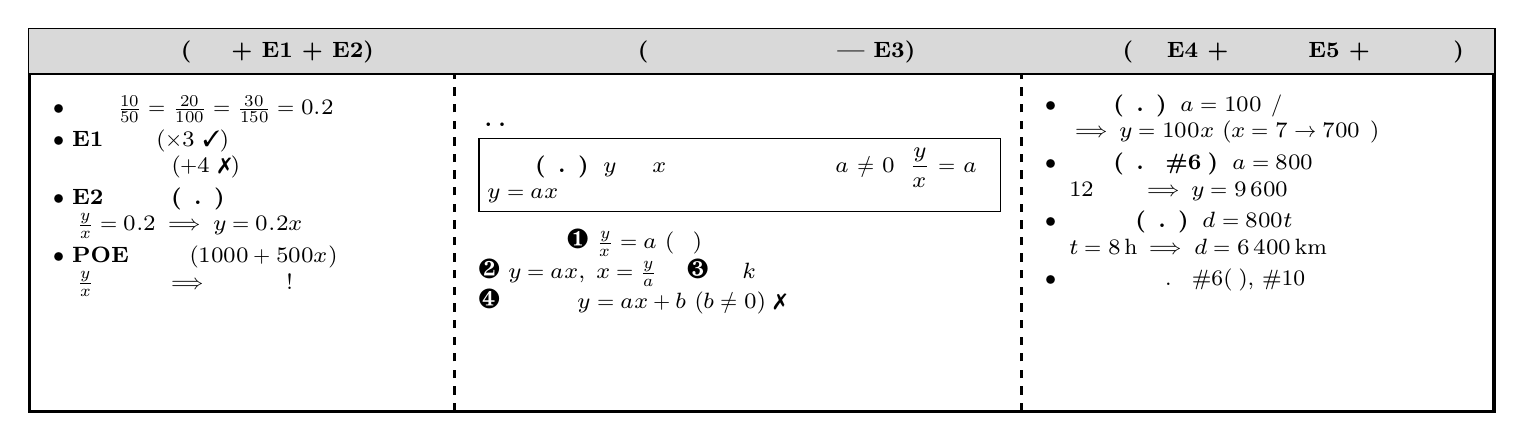
\begin{tikzpicture}[x=1cm, y=1cm, every node/.style={font=\footnotesize, text=black}]
  \draw[black, line width=1.2pt] (0,0) rectangle (18.6,4.85);
  \fill[headgray] (0,4.28) rectangle (18.6,4.85);
  \draw[black, line width=0.8pt] (0,4.28) -- (18.6,4.28);
  \draw[black, line width=0.85pt, dashed] (5.4,0) -- (5.4,4.28);
  \draw[black, line width=0.85pt, dashed] (12.6,0) -- (12.6,4.28);

  \node at (2.7,4.56) {\textbf{ផ្នែកឆ្វេង (រំលឹក + \en{E1} + \en{E2})}};
  \node at (9.0,4.56) {\textbf{ផ្នែកកណ្ដាល (ខ្លឹមសារគោលរក្សាទុកដល់ចប់ម៉ោង — \en{E3})}};
  \node at (15.6,4.56) {\textbf{ផ្នែកស្ដាំ (គំរូ \en{E4} + ប្រតិបត្តិ \en{E5} + កិច្ចការផ្ទះ)}};

  % Left zone
  \node[anchor=north west, align=left] at (0.18,4.14) {
    $\bullet$ \textbf{រំលឹក៖} $\frac{10}{50}=\frac{20}{100}=\frac{30}{150}=0.2$\\[2pt]
    $\bullet$ \textbf{\en{E1}៖} សៀវភៅ ($\times 3$ \ding{51})\\
    \hspace*{0.3cm}ធៀបអាយុបងប្អូន ($+4$ \ding{55})\\[2pt]
    $\bullet$ \textbf{\en{E2} ជញ្ជីងដៃ (ទំ.២៧)៖}\\
    \hspace*{0.3cm}$\frac{y}{x} = 0.2 \implies y = 0.2x$\\[2pt]
    $\bullet$ \textbf{\en{POE}៖} ករណី ខ ($1000+500x$)\\
    \hspace*{0.3cm}$\frac{y}{x}$ ប្រែប្រួល $\implies$ មិនសមាមាត្រ!
  };

  % Middle zone
  \node[anchor=north west, align=left] at (5.58,4.14) {
    {\muol\fontsize{8.5pt}{12pt}\selectfont មេរៀនទី៣៖ ទំហំសមាមាត្រនិងភាគរយ}\\[2pt]
    \textbf{១.១. ទំហំសមាមាត្រស្រប}\\[3pt]
    \fbox{\parbox{6.4cm}{\textbf{ជាទូទៅ (ទំ.២៧)៖} $y$ និង $x$ ជាទំហំសមាមាត្រស្រប មេគុណ $a\neq 0$៖ $\dfrac{y}{x}=a$ ឬ $y=ax$ ។}}\\[5pt]
    \textbf{ធនាគារហេតុផល៖} \cnum{1} $\frac{y}{x}=a$ (ថេរ)\\
    \cnum{2} $y=ax,\; x=\frac{y}{a}$ \quad \cnum{3} កើន $k$ ដងដូចគ្នា\\
    \cnum{4} អន្ទាក់បូក $y=ax+b$ ($b\neq 0$) \ding{55}
  };

  % Right zone
  \node[anchor=north west, align=left] at (12.78,4.14) {
    $\bullet$ \textbf{គំរូ ១ (ទំ.២៨)៖} $a=100\riel/\text{ថ្ងៃ}$\\
    \hspace*{0.3cm}$\implies y = 100x$ ($x=7\to 700\riel$)\\[2pt]
    $\bullet$ \textbf{គំរូ ២ (ទំ.៤០ \#6ក)៖} $a=800\riel$\\
    \hspace*{0.3cm}$12$ ក្បាល $\implies y = 9\,600\riel$\\[2pt]
    $\bullet$ \textbf{ប្រតិបត្តិ (ទំ.២៨)៖} $d=800t$\\
    \hspace*{0.3cm}$t=8\unit{h} \implies d=6\,400\unit{km}$\\[2pt]
    $\bullet$ \textbf{កិច្ចការផ្ទះ៖} ទំ.៤១ \#6(គ), \#10
  };
\end{tikzpicture}
\end{center}

\secstrip{២. ចម្លើយផ្ទៀងផ្ទាត់រហ័សសម្រាប់សន្លឹកកិច្ចការសិស្ស (ទំព័រ ១ និង ទំព័រ ២)}{\en{Answer Key \& Scoring Guide}}

\begin{tcolorbox}[
  enhanced, sharp corners, colback=white, colframe=black,
  boxrule=0.8pt, boxsep=1.5pt, top=3pt, bottom=3pt, left=5pt, right=5pt,
  after skip=3.5pt
]
  \fontsize{8.8pt}{13.0pt}\selectfont
  $\bullet$ \textbf{ផ្នែក \en{E1}៖} ពេលដារ៉ាអាយុ $6$ ឆ្នាំ បងសុខាមានអាយុ $\mathbf{10}$ ឆ្នាំ ($6+4=10$, មិនមែន $18$ ឆ្នាំទេ) ។ ស្ថានភាពទាំងពីរ \textbf{មិនដូចគ្នាទេ} ។\\[2pt]
  $\bullet$ \textbf{ផ្នែក \en{E2} សកម្មភាព ១ (ទំ.២៧)៖} ចំពោះ $x = 300\unit{g} \implies y = \mathbf{60\unit{mm}}$ ។ ជួរផលធៀប $\dfrac{y}{x} = \mathbf{0.2}$ គ្រប់ប្រអប់ទាំងអស់ ។ ពេល $x$ កើន $\mathbf{2}$ ដង នោះ $y$ កើន $\mathbf{2}$ ដង; សមីការគឺ $y = \mathbf{0.2}x$ ។\\[2pt]
  $\bullet$ \textbf{ផ្នែក \en{E2} សកម្មភាព ២ (\en{POE})៖}
  \textbf{ករណី ក៖} $\frac{4\,800}{6} = \mathbf{800},\; \frac{9\,600}{12} = \mathbf{800}$ (ថេរ $\implies$ \textbf{ជាសមាមាត្រស្រប} \ding{51}) ។
  \textbf{ករណី ខ៖} $\frac{2\,000}{2} = \mathbf{1\,000},\; \frac{3\,000}{4} = \mathbf{750}$ (មិនថេរ $\implies$ \textbf{មិនមែនសមាមាត្រស្រប} \ding{55} ព្រោះមានបូកថ្លៃសេវាដើមថេរ $1\,000\riel$ ធ្វើឱ្យផលធៀប $\frac{y}{x}$ ប្រែប្រួល) ។\\[2pt]
  $\bullet$ \textbf{ផ្នែក \en{E3}៖} ប្រអប់ជាទូទៅ៖ $\dfrac{y}{x} = \mathbf{a}$ ឬ $y = \mathbf{ax}$ ($a\neq 0$) ។\\[2pt]
  $\bullet$ \textbf{ផ្នែក \en{E4}៖}
  \textbf{គំរូទី ១ (ទំ.២៨)៖} $x$ ជាចំនួនថ្ងៃហួសកំណត់, $a = \mathbf{100}\riel/\text{ថ្ងៃ}$, សមីការ $\mathbf{y = 100x}$ ។ (ក) $x=7 \implies y = 100\times 7 = \mathbf{700\riel}$; (ខ) $y=1\,500\riel \implies x = \frac{1\,500}{100} = \mathbf{15}$ ថ្ងៃ ។
  \textbf{គំរូទី ២ (ទំ.៤០ \#6 ក)៖} របៀបទី ១៖ $a = \mathbf{800}\riel/\text{ក្បាល} \implies y = 800\times 12 = \mathbf{9\,600\riel}$ ។ របៀបទី ២៖ កើន $\mathbf{2}$ ដង $\implies y = 4\,800\times 2 = \mathbf{9\,600\riel}$ ។\\[2pt]
  $\bullet$ \textbf{ផ្នែក \en{E5}៖}
  \textbf{១) ប្រតិបត្តិយន្តហោះ (ទំ.២៨)៖} $a = \mathbf{800}\unit{km/h}$, $d = \mathbf{800t}$, ចំពោះ $t=8\unit{h} \implies d = 800\times 8 = \mathbf{6\,400\unit{km}}$ ។
  \textbf{២) ថ្លៃតែ (ទំ.៤១ \#6 ខ)៖} $a = \mathbf{15\,000}\riel/\text{kg} \implies y = 15\,000\times 10 = \mathbf{150\,000\riel}$ ។ បិទ \en{E1}៖ អាយុ $\mathbf{10}$ ឆ្នាំ (ហេតុផល \cnum{4}) ។
  \textbf{៣) វិនិច្ឆ័យ \en{A--D}៖} ជម្រើសត្រូវគឺ \textbf{\en{C}} ព្រោះ $\frac{14}{2}=\frac{35}{5}=\frac{56}{8}=\mathbf{7}$ ថេរ (\cnum{1}) ។
  \textbf{៤) សំបុត្រចេញ៖} (ក) $a = \mathbf{7}$, $y = \mathbf{7x}$; (ខ) \textbf{ទេ} ព្រោះមានតួដកថេរ $-2 \neq 0$ (\cnum{4}) ។
\end{tcolorbox}

\secstrip{៣. ចម្លើយលម្អិតនៃកិច្ចការផ្ទះ (សម្រាប់គ្រូផ្ទៀងនៅដើមម៉ោងបន្ទាប់ ១.២)}{សៀវភៅគោល ទំ.៤១}

\begin{tcolorbox}[
  enhanced, sharp corners, colback=panelgray, colframe=black,
  boxrule=0.85pt, boxsep=1.5pt, top=3pt, bottom=3pt, left=5pt, right=5pt
]
  \fontsize{8.8pt}{13.0pt}\selectfont
  \textbf{១) លំហាត់ ៦ គ (ទំ.៤១)៖} តាង $P$ ជាថ្លៃស្ករស $x\unit{kg}$ ។ ដោយតម្លៃសមាមាត្រស្របនឹងបរិមាណស្ករស ($y \neq 0$)៖\\
  \hspace*{0.4cm}មេគុណសមាមាត្រ (ថ្លៃស្ករសក្នុង $1\unit{kg}$) គឺ $a = \dfrac{z}{y}$ រៀល/$\unit{kg}$ $\implies$ ថ្លៃស្ករស $x\unit{kg}$ គឺ $P = a\cdot x = \mathbf{\dfrac{xz}{y}}$ រៀល ។\\[3pt]
  \textbf{២) លំហាត់ ១០ (ទំ.៤១)៖}
  \begin{itemize}[leftmargin=0.6cm, topsep=1pt, itemsep=1pt]
    \item រកចំណុះធុងប្រេងសាំងទាំងមូល (តាង $V$ គិតជាលីត្រ)៖ តាម $y = ax \implies V = \dfrac{112\,500}{3\,750} = \mathbf{30\unit{L}}$ ។
    \item តម្លៃប្រេងសាំងថ្មីក្នុង $1\unit{L}$ ក្រោយដំឡើង $210\riel$៖ $a_{\text{ថ្មី}} = 3\,750 + 210 = \mathbf{3\,960\riel/\text{L}}$ ។
    \item តម្លៃប្រេងសាំងចាក់ពេញធុង ($30\unit{L}$) នៅពេលឥឡូវនេះ៖ $y_{\text{ថ្មី}} = 3\,960 \times 30 = \mathbf{118\,800\riel}$ ។
    \item \textit{(របៀបទី ២ រហ័ស៖ ប្រាក់កើនបន្ថែមសរុប $= 210\riel/\text{L} \times 30\unit{L} = 6\,300\riel \implies 112\,500 + 6\,300 = \mathbf{118\,800\riel}$)} ។
  \end{itemize}
\end{tcolorbox}

\end{document}
